% !TEX root = robobrain.tex


\subsection{\robobrain{} for sharing knowledge}
\robobrain{} allows sharing the knowledge learned by different research groups as well as knowledge obtained from various internet sources. In this section we show with experiments how sharing knowledge improves existing robotic applications:


\subsubsection{Sharing knowledge from the Internet}
In this experiment we show that sharing knowledge from several Internet sources using \robobrain{} improves robotic applications such as path planning.  Knowledge from the Internet sources has been shown to help robots in planing better paths~\citep{beetzIcra2010}, understand natural language~\citep{coyneCosli,tellex2011understanding}, and also recently in object retrieval~\citep{guadarramaRss2014}. However, for certain robotic tasks a single Internet source does not cover many of the real world situations that the robot may encounter. In such situations it is desired to share the information from other sources to get an overall richer representation.
The \robobrain{} graph is designed to acquire and connect information from multiple Internet sources and make it accessible to robots.

In this experiment we build upon work by Jain et al.~\citep{jainsaxena2013_trajectorypreferences} for planning trajectories that follow user preferences. The work relied on object attributes in order to plan desirable trajectories. These attributes convey properties such as whether an object is sharp, heavy, electronic etc. The attributes were manually defined by the authors~\citep{jainsaxena2013_trajectorypreferences}. In practice this is very challenging and time-consuming because there are many objects and many attributes for each object.
%Jain et al.~\citep{jainsaxena2013_trajectorypreferences}  manually define attributes used by TPP.
Instead of manually defining the attributes, we can retrieve many of them from the Internet knowledge
sources such as OpenCyc, Wikipedia, etc. However, a single knowledge source might not have
attributes for all objects.
The \robobrain{} graph connects many attributes obtained from multiple Internet sources to their respective objects.
%We crawl multiple internet sources to retrieve many attributes and connect them to their respective objects in the \robobrain{} graph.


\begin{figure}
\centering
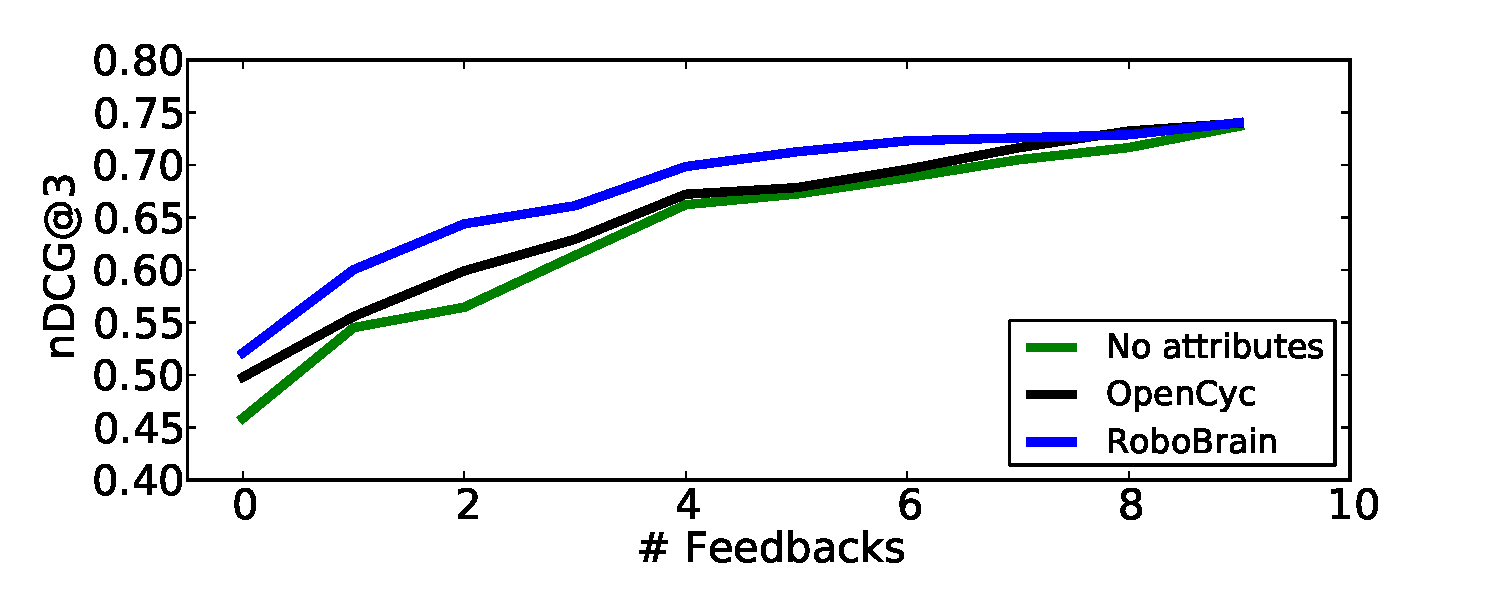
\includegraphics[width=\linewidth]{Image/internet_attributes}
\caption{\textbf{Sharing from Internet sources.} The plot shows performance of  the algorithm by Jain et al.~\citep{jainsaxena2013_trajectorypreferences} for three settings of attributes. This is an online algorithm that learns a good trajectory from the user feedback. The performance is measured using the nDCG metric~\cite{manning2008introduction}, which represents the quality of the ranked list of trajectories. \robobrain{} combines information from multiple sources and hence its richer in attributes as compared to retrieving attributes from OpenCyc alone.}
\label{fig:ndcg}
\end{figure}

Figure~\ref{fig:ndcg} illustrates the planning results when the robot does not use any attributes, when it uses attributes from a single source (OpenCyc), and when it use attributes from \robobrain{}. The planning performance is best when using \robobrain{} since it covers more attributes than the OpenCyc alone. Most importantly all these attributes are retrieved from the \robobrain{} graph with a single RQL query as explained in Section \ref{sec:applicationplanit}.


\subsubsection{Sharing learned representations}

New algorithms are commonly proposed for a problem to address the shortcomings of previous methods. These algorithms have their own learned representations. For example,  different representations  have been learned for grounding natural language~\citep{tellex2011understanding,misra2014tell,guadarrama2013grounding, MatuszekISER2012}. However, it is usually hard for practitioners to choose a single representation since there are always inputs where one representation fails but some others work. In this experiment we show that a robot can query \robobrain{} for the best representation while being agnostic to the algorithmic details of the learned representations.

Simulating the above setting, we present an experiment for sharing multiple learned representations on a natural language grounding problem. Here the goal is  to output a sequence of instructions for the robot to follow, given an input natural language command and an environment.
Following the work by Misra et al.~\citep{misra2014tell}, we train a baseline algorithm for the task of \textit{making ramen} (Algorithm A), and train their full algorithm for the task of \textit{making affogato} (Algorithm B). These algorithms assign a  confidence score (i.e., probability) to the output sequence of instructions.  We store these learned representations as concepts in the \robobrain{} graph, along with a prior belief over the correctness of the algorithms. The robot queries \robobrain{} for a representation as follows:
%\resizebox{\linewidth}{!}{
%\begin{minipage}{\linewidth}
{\small
\begin{align*}
& {\tt algParam  :=  fetch (u\{type:'GroundingAlgorithm'\})}\rightarrow \\
& {\tt \hspace*{2cm} [`HasParameters'] \rightarrow (v)}   \\
& {\tt prior \,\, n :=  fetch (\{name:n\})\rightarrow [`HasPriorProb'] \rightarrow (v)}\\
& {\tt groundings \,\, L,E :=   argMaxBy(\lambda(u,v)\rightarrow v)} \\
& {\tt \hspace*{2cm} map(\lambda(u,v) \rightarrow u(L,E,v)*prior\, u) \, \, \, algParam}
\end{align*}
%\end{minipage}
}

\medskip
In the ${\tt algParam}$ function, we retrieve all natural language grounding algorithms from the \robobrain{} graph with their parameters. This returns a list in which each element is a tuple of algorithm $u$ and its parameters $v$. The ${\tt prior}$ function retrieves the prior belief over the correctness of an algorithm. In order to ground a given natural language command ${\tt L}$ in environment ${\tt E}$, the ${\tt grounding}$ function evaluates the likelihood score for each algorithm  using their parameters as ${\tt u(L,E,v)}$. It further incorporates the prior belief over the algorithms, and returns the representation with the highest likelihood score. These set of queries corresponds to the following likelihood maximization equation:
\begin{equation*}
\mathcal{I}^*  = \argmax_{\mathcal{I},m'\in \{A,B\}} P(\mathcal{I}|E, L,  w_{m'}^* ,m')P(m')
\end{equation*}
As shown in the Table~\ref{tbl:grounding-results}, choosing a representation by querying the \robobrain{} achieves better performance than the individual algorithms.

\begin{table}
\caption{\robobrain{} allows sharing learned representations. It allows the robot to query \robobrain{} for a representation given an input natural language command. In this table the Algorithm $A$ is a greedy algorithm based on Misra et al.~\cite{misra2014tell}, and Algorithm $B$ is their full model. The $IED$ metric measures the string-edit distance and the $EED$ metric measures the semantic distance between the ground-truth and the inferred output instruction sequences. The metrics are normalized to 100 such that higher numbers are better.}
\label{tbl:grounding-results}
\centering
\begin{tabular}{l|cc}
\hline
\textbf{Algorithm} & \textbf{IED} & \textbf{EED}\\
\hline
Algorithm A & 31.7 & 16.3\\
Algorithm B & 23.7 & \textbf{27.0}\\
\robobrain{} (A+B) & \textbf{34.2} & 24.2\\
\hline
\end{tabular}
\end{table}
